% !BIB TS-program = 
%%%%%%%%%%%%%%%%%%%%%%%%%%%%%%%%%

% This is the "before the document" area, where to define parameters for the cover sheet and to include libraries

%%%%%%%%%%%%%%%%%%%%%%%%%%%%%%%%%

\documentclass[11pt]{article} 

%libraries
\usepackage{geometry}
\usepackage{float}
\usepackage{amsmath}
\usepackage{mathtools}
\usepackage{url}
\usepackage{fancyhdr}
\usepackage{graphicx}
\usepackage{multicol}
\usepackage{setspace}
\usepackage{listings}
\usepackage[numbered,autolinebreaks,useliterate]{mcode}
\usepackage{pdfpages}
\usepackage{booktabs} 
\usepackage{bigstrut}
\usepackage{bigdelim}
\usepackage{multirow}
\usepackage[nottoc]{tocbibind}
\usepackage{rotating}
\usepackage[parfill]{parskip}
\usepackage[utf8]{inputenc}
\usepackage[english]{babel}

%pagestyle
\geometry{paper=a4paper,left=30mm,right=25mm,top=40mm,bottom =30mm,headsep=20mm}

\pagestyle{fancy}
\fancyhf{}


%%%%%%%%%%%%%%%%%%%%%%%%%%%%%%%%%

% Header and Footer

%%%%%%%%%%%%%%%%%%%%%%%%%%%%%%%%%

%Kopfzeile links bzw. innen
\fancyhead[L]{\large{}}
%Kopfzeile mittig
\fancyhead[C]{\large{Master thesis proposal}}
%Kopfzeile rechts bzw. außen
\fancyhead[R]{
\includegraphics{files/TUs}}
%Linie oben
\renewcommand{\headrulewidth}{0.5 pt}

%Fußzeile mittig
\fancyfoot[C]{\thepage}


%%%%%%%%%%%%%%%%%%%%%%%%%%%%%%%%%

% Titlepage

%%%%%%%%%%%%%%%%%%%%%%%%%%%%%%%%%

%Now we start the main document body
\begin{document}

\begin{titlepage}
	\begin{multicols}{2} 
		\textbf {Technische Universit\"{a}t Berlin}\\
		Faculty:            \\ Geodesy and Geoinformation Science\\  \\
		Professor: \\
		Prof. Dr. Martin Kada\\
		\columnbreak
		\flushright
		
\includegraphics{files/TU} 
	\end{multicols}

	%Absatz
	\vspace{0.1\textheight}
	
	\begin{center}
		Master Thesis
	\end{center}
	
	%Absatz
	\begin{verbatim}
 
 
 
	\end{verbatim}
	\begin{center}
		\textbf{\Large{Proposal \\ Lunar Crater Detection using Convolutional Neural Networks}}\\
	\end{center}

	\vspace{0.35\textheight}

	\begin{center}
		\vspace{0.7cm}
		\textbf{Authors:}\\
		Tahir, Waqas \\
	\end{center}
	\begin{center}	
		\textbf{Spervisors:}\\
		Amgad Agoub\\
		Philipp Gläser\\
	\end{center}
	\begin{verbatim}
 
	\end{verbatim}
	\begin{center}
		\today
	\end{center}

\end{titlepage}

%this command is used in order to have every section in a different page, but avoid to use it!
\newpage 


%%%%%%%%%%%%%%%%%%%%%%%%%%%%%%%%%

% Table of Contents

%%%%%%%%%%%%%%%%%%%%%%%%%%%%%%%%%

%create the table of contents, figures and tables
\tableofcontents

\newpage
%%%%%%%%%%%%%%%%%%%%%%%%%%%%%%%%%

% Sections and Subsections

%%%%%%%%%%%%%%%%%%%%%%%%%%%%%%%%%

\iffalse

\section{Deep learning}


\par

\section{Supervised learning}

\par
The weight vector needs to be adjusted. The learning algorithm computes a gradient in the form of a vector for each weight which indicates the increment or decrement in error by increasing tiny amount of weight. The adjustment of weight vector is made in the opposite direction of the gradient vector. \cite{lecun_deep_2015-2}

\par
A procedure known as stochastic gradient descent is widely used by practitioners. In this procedure an input vector is shown for some examples then outputs, average gradient and errors are computed and weights are adjusted accordingly. This process is iterated for small set of multiple examples taken from training data set until the average of objective function does not further decrease. After training, the machine's performance ability is measured by feeding a test data set. This is completely new data set to machine and it produces sensible outputs from the input that it has not seen during training.

\section{Modern History of Object Detection}
Object detection has greatly inproved over the last few years. The era of deep learning had a major breakthrough when ~\cite{krizhevsky_imagenet_2012} won the ImageNet  \cite{lecun_deep_2015} 

\section{Cut lines}
Keeping in view the achievements of Mask R-CNN over previously developed algorithms, we decided to test this algorithm on lunar crater dataset. The dataset consists of 4 million images. Figure \ref{fig:Mask R-CNN results on the COCO test set.} shows the result of Mask R-CNN on COCO dataset. Faster R-CNN was extended for pixel level segmentation.

\par
Machine learning methodology becomes handy over classical object detection approaches when it comes to detecting objects from different datasets on which algorithm was not trained. In classical computer vision methods, the images are needed to be ---------- Machine learning algorithm requires labeling on of the dataset. 
 


\section{Introduction}
Studying impact craters present a valuable information about the geology of planets and characteristics of the surface.

\par
 Small and shallow craters can be analyzed from the images with high incidence angle (\textgreater70°).

\par
One single image taken from LRO could have several craters of different diameters. Manual detection takes a lot of time and man power with required skills. In last two decades, detecting craters manually was no longer an optimal solution because of several reasons like as mentioned earlier, manual detection of craters is a laborious work with involvement of man power. Another major drawback is that only qualified individuals can perform detection process. When technology is advanced enough that this laborious task can be handed over to a machine then implementing an algorithm for the automatic detection of craters would not only save time but also dependency on skilled individuals to carry out this task. 

\par
Earlier this decade, development in computer graphical units made it possible to process big data. This created an opportunity for scientists to test machine learning architectures for object detection. Convolutional Neural Networks also known as CNNs or ConvNets are an architecture of supervised machine learning model that have proved their success by winning Large Scale Visual Recognition Challenge (ILSVRC-2010) competition which was composed of 1.2 million high-resolution images. \cite{krizhevsky_imagenet_2012} achieved top-1 and top-5 error rates of 37.5\% and 17.0\% respectively. This success gave rise to ConvNets architectures and since then scientists have been working to increase the object classification speed of such algorithms.

The aim is to develop a CNN architect and test its performance on automatically crater presence and edge detection by performing a series of computations. Mask R-CNN (Mask Region Convolutional Neural Network) was presented in 2017 where the goal was a pixel level classification of each pixel into fixed set of categories. The example image of such method is shown in figure \ref{fig:Mask R-CNN results on the COCO test set.}. Other than CNNs, there is another way to detect an object, YOLO (You Look Only Once) i.e. does not classify objects as accurately as CNN because in YOLO each object in the image is assigned to grid cell that contains the object's midpoint. Each grid detects one object only regardless the number of bounding boxes. It is faster than CNN because it takes object detection as a regression problem to spatially separated bounding boxes and class probabilities associated with it, these classes are predicted with a single neural network in one evaluation. One of the example of YOLO result is also shown in Figure  \ref{fig:YOLO running on sample artwork and natural images from the internet.}.

\begin{figure}[H]
	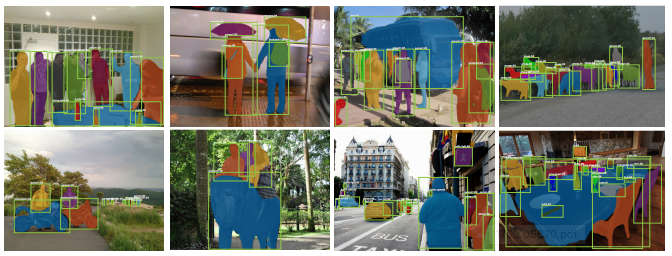
\includegraphics[width=\linewidth]{files/mask_R-CNN/results.jpg}
	\caption{Mask R-CNN results on the COCO test set.}
	\label{fig:Mask R-CNN results on the COCO test set.}
\end{figure} 

\begin{figure}[H]
	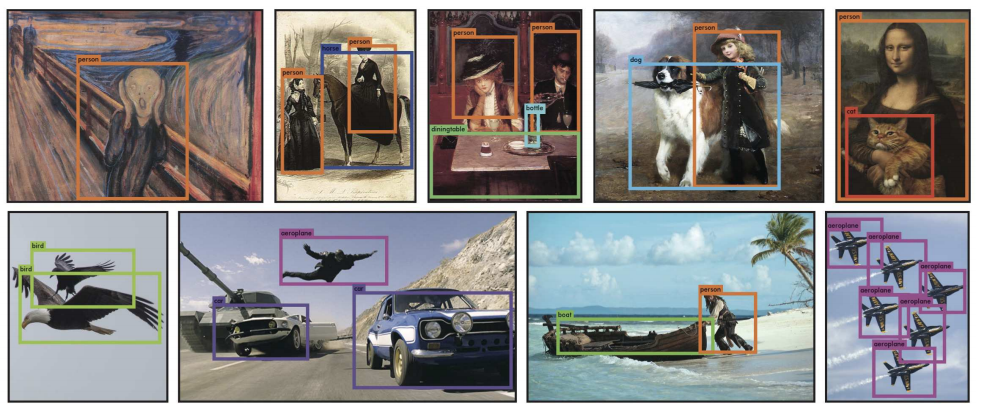
\includegraphics[width=\linewidth]{files/yolo/results.jpg}
	\caption{YOLO running on sample artwork and natural images from the Internet.}
	\label{fig:YOLO running on sample artwork and natural images from the internet.}
\end{figure}

Figure \ref{fig:YOLO running on sample artwork and natural images from the internet.} shows YOLO results on Picasso and People-Art datasets. In this image it can be seen that YOLO has predicted a person as an airplane. Even though it is mostly accurate.
\fi

\section{Introduction}
Studying impact craters present a valuable information about the geology of planets and characteristics of the surface. Computation of crater density has provided a gateway for the establishment of evolution of planet terrains chronologically \cite{martins2009crater}. This study provide not only the information about geological processes of the planet but also the history of our solar system. According to geologists impact craters are the only modifying and surface forming process for other planets and moons of all planets \cite{koeberl1994african}. Impact craters have also been a useful source of information for planetologist in providing the relative age of surfaces. If the relationship between crater size and impact energy is known and flux caused by the impact is understood then craters with larger densities indicate older surfaces \cite{ivanov2002comparison}.

Various processes alter crater populations specially of those with smaller diameters \cite{opik1965mariner} more often in planets with an atmosphere. This results deviations in crater size-frequency distributions (CSFD). Factors like deceleration, ablation, fragmentation of meteors while passing through the atmosphere before striking the surface, the effect of target properties on scale of crater formation and postformation changes of craters by erosion and deposition.Therefore, crater counts with relatively smaller diameters (i.e. d $<$ 1 km) are at a larger risk of representing an age which could be misinterpreted if the modeled production function does not take into account the factors responsible for altering CSFD in an observed range of diameter \cite{hartmann1981chronology}.Moreover, several factors may lead to surface age as well as statistical uncertainties because smaller crater's identification is prone to certain biases such as resolution limits, illumination effects, compact crater count areas or limited number of craters \cite{soderblom1970distribution}.

Modeling of impact craters depends on the knowledge of age-dated lunar samples with correlation to observed CSFDs \cite{williams2018dating}. Chronology is a system composed of two elements such as a production function describing the CSFD shape and a chronology function which is related to the accumulation of craters density to absolute time. Both of these functions collectively provide a predicted CSFD or isochron for a given time length a surface has been under crater strikes. This is valid for lunar surface as Moon has no atmosphere. This chronology can also be applied to other solar system objects but with an addition of factors such as impactor flux and surface gravity \cite{ivanov2002comparison}.

If CSFD and the diameter of crater is known then age of the lunar surface can be determined using both of these parameters. It is only possible to determine the age of the same area where crater count has been performed. There are production functions proposed by planetary scientists which provide an approximation to surface age if CSFD and crater diameters are known. The examples of such functions are Hartmann Production Function (HPF) and Neukum Production Function (NPF).

Crater-counts gives the frequency of crater distribution of a certain area. This can be performed by counting craters manually. This task could not only be time consuming but also expensive and labor intensive depending upon the number of images and amount of craters present in images. Satellites are the source of images which provide opportunity to count craters depending on the type of cameras on board. Also number of craters in a certain area may change with a passage of time which would mean that the same task for the same surface has to be performed again. This is a challenging requirement, therefore in scope of this thesis the target is to automate crater detection which would be much faster, cheaper and also efficient. The efficiency of crater detection would be tested in two ways. First, the automatic prediction will be compared against manually detected craters and secondly the age approximation would be compared to the already known surface age. Analysis of craters will provide required diameter and these parameters (CSFD and diameter) as mentioned before would lead to age determination.

Since early 2000 many missions and satellites have been deployed to Moon for research purposes including crater studies. LRO (Lunar Reconnaissance Orbiter) is one of the satellites on lunar mission operated by USA and is collecting lunar images since 2009. LRO has gathered millions of images since its launch. Lunar Reconnaissance Orbiter Camera (LROC) was specifically designed for the assessment of meter and smaller scale features to help carry out safety analysis for future lunar landing sites on moon including polar region. The Narrow Angle Cameras (NAC) mounted on LRO are able to detect craters with diameter of 2.5 m or greater \cite{robinson2010lunar}. It is common to find craters less than 100 m in diameter on lunar surface \cite{robinson2010lunar}.

A single image size taken from LRO is upto 5064x52224 pixels with a resolution of 1.009. The data is available publicly and can be seen or downloaded through this link \textit{(http://wms.lroc.
	asu.edu/lroc/)}. 
Such images cannot be processed without a competitive machine. There are methods developed to perform image processing tasks which are highly dependent on a machine's memory and performance. Therefore, developing techniques without advancement in computer technology was simply not enough. This problem was already known and therefore it lead to the development of Graphical processing unit (GPU). A GPU performs quick math calculations and frees the space for CPU to do other tasks. Unlike CPU it has thousands of cores designed for multi-tasking. A much needed hardware to perform computationally expensive calculations without exhaustion. 

In 2000s many companies like Intel, Nvidia and AMD/ATI stepped into the race of manufacturing faster GPUs and dominated market. This competition continues till today and GPUs are becoming more and more powerful. Meanwhile, the need for GPUs is also increasing because of big data processing needs. Nvidia introduced a chip capable of programmable pixel shaders i.e. compute color, position, depth or stencil of a pixel, the Ge-Force 3. A short program could now process each pixel before projecting it to the screen, this processing included but not limited to addition of image textures. By 2002 ATI Radeon 9700 the world's first Direct3D 9.0 accelerator was introduced my Microsoft containing support for multiple render targets, floating point texture formats, multiple-element textures and stencil buffer methods. In 2010 Nvidia began a partnership with Audi to power car dashboards. This mainly increased the functionality of navigation and entertainment systems. In 2014 the PS4 and Xbox One were released powered by GPUs based on AMD's Radeon HD 7850 and 7790. Lately RTX was released by Nvidia with the aim of enabling real time ray tracing. This was a new development in computer graphics for generation of interactive images reacting to lighting, reflections and shadows. RTX also includes artificial intelligence (AI) integration like enhancing video processing, graphics and images directly into applications. Today, parallel GPUs are making complex computations in the fields of oil exploration, machine learning, image processing, 3D reconstruction, statistics and even in stock market for stock rates determination. 

In the past automatic detection of craters turned out to be a difficult task in cases when rims were not clear or overlapped or if image is noisy \cite{sawabe_2006}. Multiple automated methods were presented by \cite{sawabe_2006} using the data acquired by Clementine and Apollo. One of the methods was to thin down a set of edge pixels to one pixel using Hilditch's thinning algorithm. The lines were then connected depending upon the direction and length. If the resultant lines were closed with roundness more than 0.8 then lines were regarded as crater. During last decade new techniques have been developed in object detection, localization, semantic segmentation and instance segmentation, these techniques are referred to as Dee. Like mentioned earlier, these methods can now put into application because of GPUs of today, which is not only capable of performing computationally intensive tasks but also shortens the amount of processing time.

In the scope of this thesis, a deep learning model will be applied to solve the problem of automatic crater detection which will reduce the cost of detection by eliminating skilled man power and saving time. In this model images will be subjected to convolutional operation (mathematical element wise-multiplication) and such type of neural networks are known as Convolutional Neural Networks or CNNs. These are architectures of supervised machine learning model that have proved their success by winning Large Scale Visual Recognition Challenge (ILSVRC-2010) competition which was composed of 1.2 million high-resolution images. \cite{krizhevsky_imagenet_2012} achieved top-1 and top-5 error rates of 37.5\% and 17.0\% respectively. A CNN algorithm will be customized, trained and tested for lunar crater detection. The proposed algorithm will be applied to images taken by Lunar Reconnaissance Orbiter irrespective of specific camera limitations. The outcome of this model will be a trained version of this model also called as a checkpoint with minimum loss function. This trained model will be tested on lunar images and it will give predictions of craters in those images (pixel wise detection of crater in an image). This will provide the frequency of craters. As mentioned before, determination of diameters of craters would require post-processing, afterwards both of these values (crater frequency and diameter) will serve as an input to chosen lunar production function. This production function will be plotted to find out the age of target surface.

\section{Background}
But why is it important to study craters? The fact that studying the surface of other planets is a source of learning about our own planet. How crater impacts can effect the life on Earth, climatic change globally and possible consequences of what can happen to our planet in an extreme case. Finding age from crater-counts is a commonly accepted method. This will be achieved by a deep learning model and results will be utilized to find out the lunar surface age. As mentioned before, crater-counts provide a less expensive way to find out the age of surface as compared to Radioactive Age-Dating. As for the second, a rock sample is needed and age can only be determined for a specific area whereas by crater-counts it is possible to find out the age of a larger area.

The problem of detecting objects could be complicated specially when object background is complex. With advancements in computer technology it was no longer optimum to rely on manual detection of objects. With big data and challenge of solving tasks in limited time, it was required to develop a mechanism that could solve such tasks in faster time compared to expensive manual operations and meanwhile limit man power. This gave rise to research in deep learning approaches to solve this problem.

Deep learning models composed of multiple processing layers learn the representation of data with numerous levels of abstraction by deep learning. These methods have made dramatic improvement in state of the art visual object recognition, speech recognition, object detection and many other areas such as genomics and drug discovery. Deep learning uses backpropagation algorithm to indicate how a machine should change its internal parameters of each layer from representation in the previous layer. This allows learning of machine to correctly represent i.e. patterns in an input.

Deep learning methods are the representations of multiple levels obtained by composing non linear modules such that each module transform the representation from one level to a higher level making it more abstract. Composition of such transformations makes it possible to learn complex functions. For classification, it is performed in different layers. The image is in the form of an array of pixel values, typically the first layer represents presence or absence of edges on specific locations in image.  The second layer detects a shape by visualizing edges. The third layer may densify the shape into more prominent features and later layers make use of these computations to detect objects as a resultant of combination of shapes.

Object detection and classification can be performed in supervised machine learning. In a typical supervised machine learning method a system is built that can classify different objects or animals then first it is required to have a labeled data set of such objects. For example to categorize horses and people, it is needed to have a data set which will consist of labeled images containing horses and people. This dataset would be required to train the machine about learning that how horses and people looks like so that it can classify the categories. The algorithm then outputs a vector of scores for each category. To get the category rightly identified, it is required to have the highest score for desired category out of all categories. This is not likely to happen without training of the algorithm. It is needed to compute a loss function that calculates the distance or error between the output scores and desired pattern of scores. This function helps algorithm to adjust its internal parameters that could be changed to reduce this error. These parameters are commonly referred to as weights and are real numbers.


\iffalse
In this technique an algorithm is trained by labeled images for desired classes of objects. The performance is then evaluated and tested using labeled images. The dataset is divided into 80\% training and 20\% test data. Labels are created by drawing a box around the object called a bounding box. The processes of supervised machine learning will be discussed in the later sections.
\fi

\subsection{Bounding Box Proposal}
In object detection, a bounding box (also referred to as region of interest or box proposal) shows the existence of object. It is a rectangular region of the input image containing the object. Bounding boxes can be generated by some heuristic search methods such as finding region proposal by objectness, region proposal network (RPN) or by selective search method.
A bounding box can be either represented by storing its two corner coordinates $(x_0, y_0, x_1, y_1 )$  or most commonly by storing its center location along  with width and height such $(x, y, w, h)$. A bounding box is generated on the basis of confidence score that how likely an object exists inside the box. The difference between two bounding boxes is usually measured as the L2 distance of their vector representations. Another simplest way is to compare the images by taking pixelwise difference and summing up all the differences. To perform such procedure, given two images can be represented as vectors $I_1, I_2$ then L1 can be computed as:

\begin{align*}
d_1 (I_1, I_2) = \sum_{p} \left| I^p_1 - I^p_2 \right|
\end{align*}

\begin{figure}[H]
	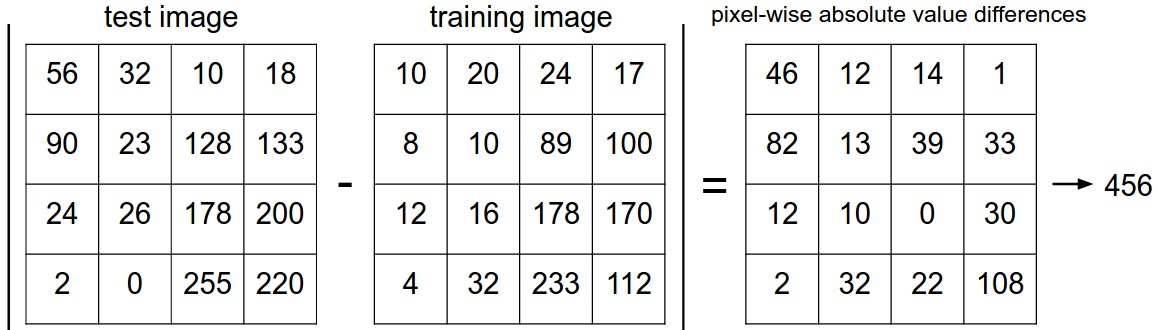
\includegraphics[width=\linewidth]{files/nneg.jpeg}
	\caption{Example of two images which are represented as vectors and pixelwise difference is calculated to compare both images with L1 distance. This example shows one color channel. All the pixel-wise differences are added to denote a single digit value. If this value is close to zero then it indicates that images are identical. A large value shows that both images are very different.}
	\label{fig: Example of two images which are represented as vectors and pixel-wise difference is calculated to compare both images with L1 distance. This example shows one color channel. All the pixel-wise differences are added to denote a single digit value. If this value is close to zero then it indicates that images are identical. A large value shows that both images are very different.}
\end{figure}

The difference between bounding boxes can also be measured by the L2 distance. Similar like L1, images are represented in a vector form. $w$ and $h$ can be log-transformed before calculating distance. L2 has the geometric representation of computing euclidean distance between two vectors as:

\begin{align*}
d_2 (I_1, I_2) = \sqrt{\sum_{p} \left( I^p_1 - I^p_2 \right)^2}
\end{align*}
 
In simple words this operation also computes the pixelwise difference like L1 but here all the differences are squared then added and finally equation is subjected to square root. Difference in measurement between both metrics differs in a way that L2 prefers many medium disagreements to one big one when it comes to difference between vectors.
 
In case of multiple bounding boxes a common algorithm to merge them is non maximum suppression (NMS). A bounding box that overlaps another one having higher confidence score with a factor such as its intersection over union (IoU) is greater than IoU threshold, is removed. Intersection over union provides similarity between two bounding boxes. ${\textit{Area of Overlap}} /{\textit{Area of Union}} = IoU
$. The bounding boxes play an important role in setting up dataset for the algorithm. Learning of the algorithm largely depends on correctly placed bounding box on the object.

With sliding windows, a bounding box can be attained but it may not properly fit the object. With bounding box and stride size, it might be only able to cover a part of the object and not the complete object. This problem can be solved using an approach developed by \cite{redmon_you_2016} where a picture is divided into multiple grids and an image classification and localization algorithm is applied to each grid. Every grid has a label $y$ which represents some parameters as shown below:

$$
y =
\begin{bmatrix}
p_c\\
b_x\\
b_y\\
b_h\\
b_w\\
c_1\\
\end{bmatrix}
$$

where $p_c$ is whether or not there is an image, $b_x, b_y, b_h$ and $b_w$ is to specify bounding box, $c_1$ is object class (i.e, craters). If there is no crater then $p_c$ will be zero and hence the entire vector is to be dropped. When $p_c$ = 1, it represents there is a crater and all the bounding box parameters would specify position of this box and hence the value of $c_1$ would be 1. Each grid cell will have this output vector $y$. The idea is to feed an input image and run forward pass (convolution, max pooling and relu) to get this output vector $y$.

The evaluation of object detection algorithm can be performed using $IoU$. As mentioned before, it gives the ratio between area of overlap and area of union. So if the algorithm outputs a bounding box which does not properly fit the ground truth bounding box representing the object then by convention the answer is taken correct if $IoU \geq 0.5$. If predicted and ground truth bounding boxes overlaps perfectly then IoU would be 1. The higher the IoU, the more accurate the bounding box is.

\subsection{Linear Classification}
It is one of the simplest technique to classify an object. Eventually it will be extended to the entire Convolutional Neural Network. It has two major components. One is score function which does the mapping of raw data to the class scores and other one is a loss function that defines how different predicted score is from the ground truth labels. Typically loss function is higher initially and thus required to be minimized with respect to the score function parameters. This minimization is also referred to as optimization. 

To define a score function which is the first component of linear classification, it is required to have information about number of images $\boldsymbol{N}$ with dimension  $\boldsymbol{D}$ i.e. the size of image (pixels and channels) and distinct categories $\boldsymbol{K}$ which are the number of classes. A simplest possible function for linear mapping:

$$
f(x_i, W, b) = Wx_i + b
$$

Here $x_i$ is the image which is flattened out to a single column vector of shape $[D \times 1]$. $\boldsymbol{W}$ is of size  $[K \times D]$ and is often referred to as weights, whereas $b$ is called bias vector with size  $[K \times 1]$. Multiplication of matrices $Wx_i$ gives separate classifiers in parallel where each classifier represents a row of weight matrix. The goal is to set the weights and bias parameters in a way that the output score match the ground truth labels of training data set as such that the correct classes has higher score than the incorrect classes.  

\subsection{Normalization}

\subsection{Neural Network Overview}
In supervised machine learning object detection task can be achieved using different approaches. There are various architectures based upon statistical functions. A neural network is made up of neurons having learnable weights and biases. It means that during training process, weights and biases can be updated. A neuron in an artificial neural network is referred to a mathematical function. It receives inputs which can also be output of neurons from a previous layer, weighs each input and sum them up. A weight shows the strength of connection of one neuron to another neuron in next layer. Every neuron has a bias and it determines if the neuron is activated or not. Biases are added to the product of weight and value of neuron. Each neuron is fully connected to all the neurons of previous layer. These neurons do not share any connection within a single layer. The last fully connected layer is referred to as "output layer". The network takes an input and computes the output by taking a dot product. The entire network takes raw image pixels and presents an output in the form of a digit representing the class score for an object. Output layer represents the class scores. It expresses a single differentiable score function. There could be few to many hidden layers and a fully connected layer that has a loss function i.e support vector machine (SVM) or softmax. A typical neural network architecture is shown below:

\begin{figure}[H]
	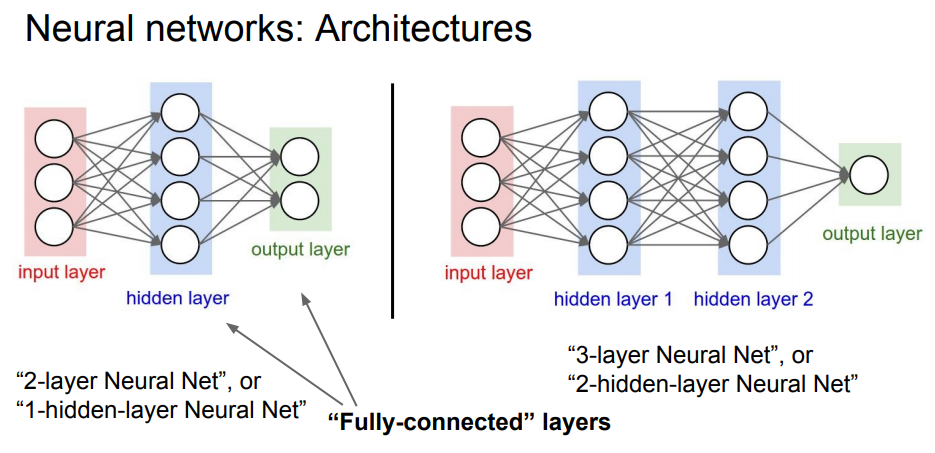
\includegraphics[width=\linewidth]{files/NN.jpeg}
	\caption{A typical Neural Network architecture}
	\label{fig: Neural Network architecture}
\end{figure}

Artificial Neural Networks are very similar to convNets but they do not convolute on an image through a filter thus leading to many more parameters as compared to CNN i.e. in CIFAR-10 dataset, images are of 32x32x3 (width, height, 3 color channels). That means in an input image of size 32x32x3, an Artificial Neural Network would have 3072 weights. These weights tend to increase with size of image.

\subsection{Convolutional Neural Network Overview}
Just like Artificial Neural Networks as shown in Fig \ref{fig: Neural Network architecture}, convNets are also made up of neurons consisting of weights and biases which are learnable. Each neuron receives an input then performs a dot product and optionally follows it with a non-linearity. The entire network represents a single differentiable score from the raw image input to the output score. Last fully connected layer has a loss function which represents the error score. This entire process is referred to as forward pass. In convNet, the architecture assume inputs as images which provides flexibility of encoding certain properties. This greatly reduce the amount of parameters to learn and make forward pass more efficient. The layers of convNets have neurons arranged in 3 dimensions (width, height, depth). The neurons in a layer are not connected to all of the neurons in a previous layer like in an Artificial Neural Networks, instead they are connected to only small region of previous layer. The output results into a single vector of class scores by reducing the full image.

\subsection{Concept of layers in CNNs}
Following are the types of layers in a Convolutional Neural Network:

\subsubsection{Convolutional layer}
Lets suppose there is a 2D input image of size 6x6. A filter convolves through the image to extract an output image with desired features. The filter (which is also a matrix) could be of size lets say 3x3, extracts certain features of the image. This process is known as convolutional operation because filter convolve through the image. In example, it would look as shown in fig: \ref{fig:Convolutional Operation}

\begin{figure}[H]
	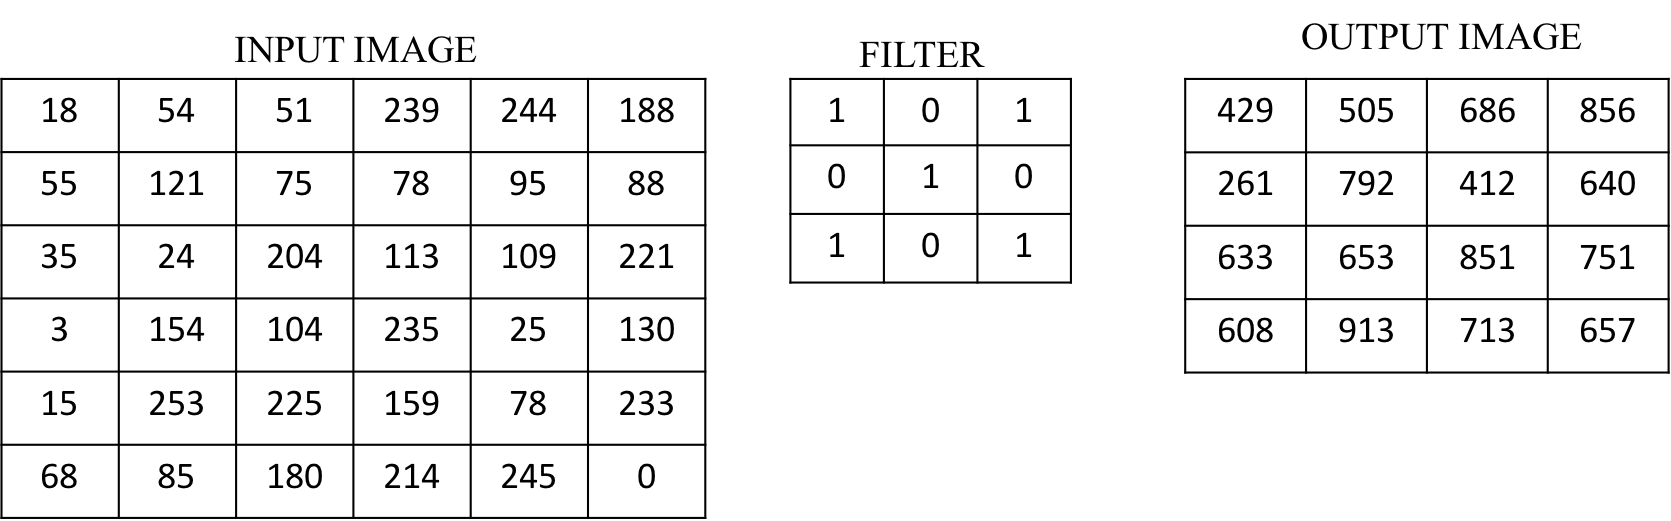
\includegraphics[width=\linewidth]{files/cnn_architecture/conv.png}
	\caption{Convolutional Operation}
	\label{fig:Convolutional Operation}
\end{figure}

In fig: \ref{fig:Convolutional Operation} the output 429 in 4x4 matrix is obtained by addition of element wise multiplication of the filter with top left 3x3 portion of the input image. Then filter jumps to next pixel and other values are obtained (stride is taken as 1). Output size can be calculated using eq.

\begin{equation}
\frac{n+2p-f}{s}+1 \times \frac{n+2p-f}{s}+1
\end{equation}

In the above example $n$ equals 6 as image is 6x6 and $f$ is 3 because of 3x3 filter size, $p$ is padding which equals 0 and $s$ stands for stride which is 1, inserting values in this equation would give us the size of output which is a 4x4 matrix.

\subsubsection{Pooling layer}
An input image could be large which increases the amount of parameters and introducing a pooling layer helps to reduce the number of parameters. Most commonly used type of pooling is max pooling. Fig \ref{fig:Pooling Operation} shows an example of max pooling with stride and filter size of 2. The idea is to keep the high values in each quadrant because the highest number represents a particular feature and in the example shown in Fig \ref{fig:Pooling Operation}, number 6 is the highest value in this quadrant. It means that the most activated pixel in this quadrant is 6 and same goes for other quadrants. The high values are preserved and lower ones are dropped out which are not as activated. Another pooling layer type is average pooling where averaged output of all the pixels is preserved. As it can be seen in the example below that pooling has reduced a 4x4 matrix to just 2x2 matrix, significant amount of parameters are reduced, in addition pooling may also help in reducing overfitting. The resultant matrix after a pooling operation can be obtained from the eq.(1) 

\begin{figure}[H]
	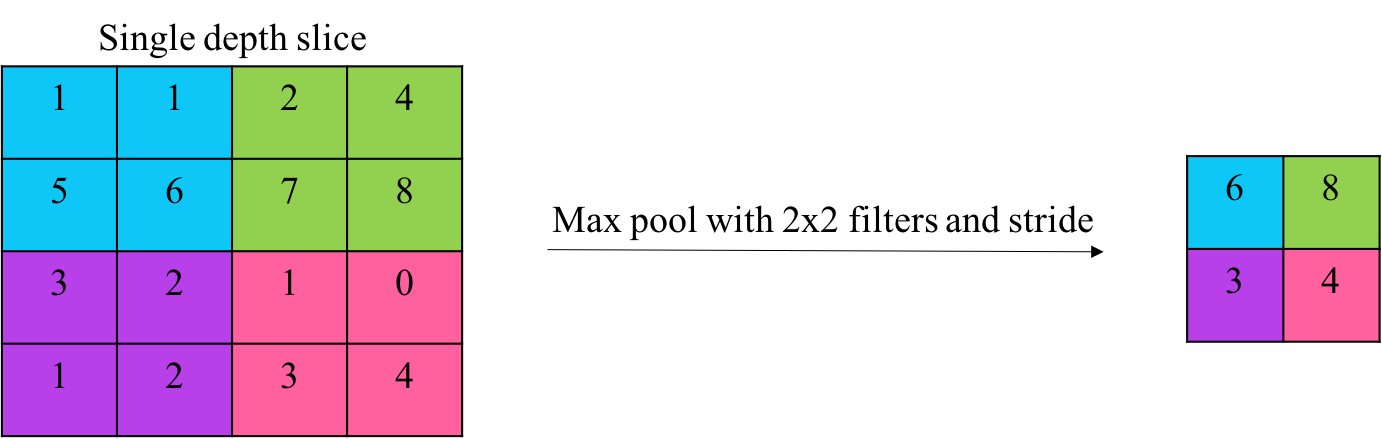
\includegraphics[width=\linewidth]{files/cnn_architecture/pooling.png}
	\caption{Pooling Operation}
	\label{fig:Pooling Operation}
\end{figure}


\subsubsection{Fully Connected layer}
After multiple convolution and pooling operations, finally an output can be generated in the form of a class. Convolution and pooling layers only extract the features and reduce amount of parameters from the input images. Fully connected layer (FC layer) is applied at the end to generate the required output equal to the number of classes. There can be multiple FC layers to further minimize the amount of parameters. In convolution the resultant is generation of 3D activation maps whereas the intention is to know whether the image belongs to a particular class or not. The output layer (which generates the class scores) has a loss function and once the forward pass is completed, backpropagation begins to update biases and weights for loss and error reduction. An overview of the architecture is shown below:

\begin{figure}[H]
	\centering
	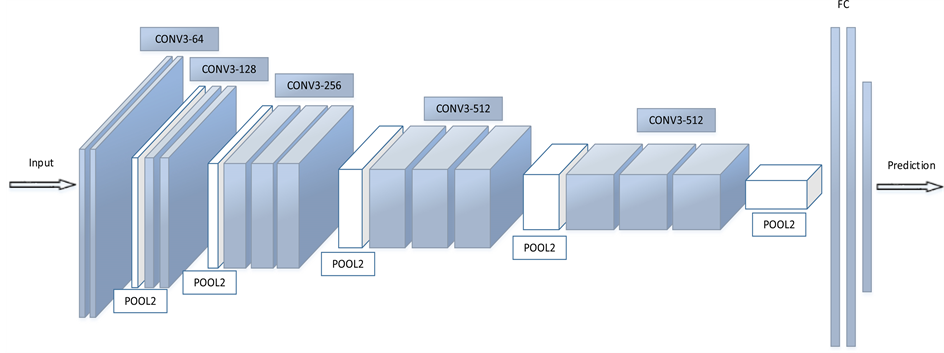
\includegraphics[width=\linewidth]{files/cnn_architecture/arch.png}
	\caption{Convolutional Neural Network Architecture \cite{2016face}}
	\label{fig: CNN architecture}
\end{figure}


%\section{Research Question}
%\begin{enumerate}
%	\item How to evaluate the performance of algorithm?
%\end{enumerate}


\section{Related Work}
Most of the craters are formed as the result of meteoroid impacts. The relative formation age of local area of planet could be estimated when frequency of size distribution of meteoroids and its time variations are known. \cite{sawabe_2006} proposed an algorithm that did not depend on cameras, spatial resolution or sun illumination. It also did not require to tune any parameters either. This algorithm was improvement to their own previously proposed algorithm. Their previous method did not include pyramid representation of the image which was included in later method and thus improving accuracy and reducing processing time. The algorithm was applied on images acquired by Clementine and Apollo under different solar elevation. The accuracy was more than 80\% compared to the manual detection results \cite{sawabe_2006}. Accuracy rate was validated by comparing with crater count results of \cite{neukum1975cratering}. In 2009 \cite{martins2009crater} performed Viola and Jones (2004) algorithm on Mars dataset gathered by the Mars Orbiter Camera onboard Mars Global Surveyor probe. In this paper author claims that no such method existed that is satisfactory for craters detection.


The idea of machine learning existed well before early 2000s but because of lack of powerful GPU it was not possible to process the intense computation. In last decade, object detection techniques have been improved considerably. In 2013 a method was developed that refined the object detection performance from previously used approaches. The idea was to combine region proposals with CNN's and the method was referred to as R-CNN \cite{girshick_rich_2013}. Since then pixel level processing advancement in the algorithm has been made and in 2017 a team of Facebook researchers came up with a new algorithm that contributed to reduced processing time and increased accuracy (up to 99\%) \cite{he_mask_2017}. They came up with a method that does not only detect an object but also generates a high quality segmentation mask for each instance \cite{he_mask_2017}. 

\par
YOLO (You Look Only Once) is another method which was developed with an intention to detect objects at a greater speed than existing algorithms. YOLO lacks state of the art object detection accuracy achieved by other CNN algorithms i.e. Faster R-CNN and Mask R-CNN. But as it states you look only once, YOLO detects an object very quickly as compared to Mask R-CNN but it struggles to localize some objects, specially small ones ~\cite{redmon_you_2016}. This is because of its spatial constraints on bounding box predictions as every grid cell can have only one class.

%\subsection{Dataset}
%For training and testing of model. The dataset is taken in the form of images from LRO in 2 different formats: grayscale and RGB. These images are of moon and consists craters of different sizes.


\section{Methodology}
The dataset which is in the form of gray scale lunar images is taken from lunar reconnaissance orbiter camera (LROC) archive \textit{http://wms.lroc.asu.edu/lroc/search}. Firstly, craters in images will be labeled. Every image will be subjected to image augmentation. This is done to achieve better training for the algorithm. Augmentation creates multiple images out of one image which means increased dataset and that let algorithm to have more training data and thus achieve better performance on test data. Most commonly used methods are mirroring and random cropping. Here in the dataset there are no RGB images hence color augmentation can not be performed.

\par
Once this dataset is labeled and augmented then next step is to utilize this datset for training of the algorithm. In this process the selected amount of filters convolute over the image and outputs a layer with detected features. All the filters detect particular features and outputs a layer as shown in Figure \ref{fig: CNN architecture}. Number of layers generated are equal to amount of filters. These layers are then subjected to pooling function to downsize image and get the neurons of highest activation. A fully connected layer is the aggregation of all the layers followed by a loss function to determine if the image contains craters or not. Loss function determines the error in percentage and a process of back propagation adjusts the weights to minimize the error. After the detection is made with a minimal error possible, it would be interesting to come up with the evaluation method for challenging the performance of this algorithm.  

\newpage

%%%%%%%%%%%%%%%%%%%%%%%%%%%%%%%%%

% Bibliography

%%%%%%%%%%%%%%%%%%%%%%%%%%%%%%%%%

	
\bibliographystyle{apalike}
\bibliography{mybib}


\end{document}
